\section{Pattern Matching}

Pattern matching adalah proses menemukan kemunculan satu pola atau lebih di dalam data yang lebih panjang, umumnya berupa string, dokumen, atau aliran teks. Pada dasarnya, masalah ini muncul ketika sistem harus menentukan apakah suatu fragmen teks cocok dengan pola tertentu, lalu pada tahap lanjutan mengukur posisi, jumlah kemunculan, atau tingkat kemiripan pola tersebut. Dalam literatur, pattern matching menjadi fondasi bagi banyak teknik pencarian string klasik seperti Knuth-Morris-Pratt, Boyer-Moore, Aho-Corasick, dan Rabin-Karp \cite{knuth1977fast,boyer1977fast,aho1975efficient,karp1987efficient}.

\begin{figure}[H]
    \centering
    
\includegraphics[width=0.9\linewidth]{pattern-matching.png}
    \caption{Gambaran umum proses pattern matching pada teks.}
    \label{fig:pattern-matching-overview}
\end{figure}

Secara umum, pattern matching dapat dipandang dari beberapa sudut pandang. Pada exact matching, pola dianggap cocok hanya jika string yang diperiksa identik dengan pola yang dituju. Pada approximate matching, sistem tetap menerima perbedaan tertentu selama jarak atau skornya masih berada dalam ambang yang ditetapkan. Pada multi-pattern matching, sistem mencari banyak pola sekaligus dalam satu teks, sedangkan pada rule-based matching, sistem memakai aturan sintaks tertentu, misalnya ekspresi reguler, untuk menangkap bentuk teks yang lebih kompleks. Klasifikasi ini penting karena tiap pendekatan memiliki karakteristik biaya komputasi, tingkat presisi, dan fleksibilitas yang berbeda.

Tipe pencocokan pola juga berbeda dalam cara menangani variasi teks. Exact matching unggul ketika daftar pola sudah jelas dan tidak banyak distorsi, sedangkan approximate matching lebih sesuai untuk data yang noisy atau sengaja dimanipulasi. Multi-pattern matching dibutuhkan ketika jumlah pola sangat banyak dan semua pola harus diproses dalam satu lintasan, sementara rule-based matching dipakai untuk menangkap struktur teks yang tidak dapat direpresentasikan hanya dengan daftar kata kunci. Dalam konteks aplikasi ini, variasi penulisan seperti penyisipan angka, perubahan huruf visual-similar, dan pola kata tertentu membuat pendekatan yang dipakai tidak bisa bergantung pada satu jenis pencocokan saja.

Algoritma yang umum digunakan dalam pattern matching memiliki strategi yang berbeda-beda. Knuth-Morris-Pratt memanfaatkan informasi prefix untuk menghindari pemeriksaan ulang karakter yang tidak perlu, Boyer-Moore memakai heuristik pergeseran dari sisi kanan pola, Aho-Corasick membangun automaton untuk pencarian banyak pola sekaligus, dan Rabin-Karp menggunakan hashing untuk membandingkan jendela teks dengan pola \cite{knuth1977fast,boyer1977fast,aho1975efficient,karp1987efficient}. Pilihan algoritma biasanya dipengaruhi oleh panjang teks, jumlah pola, kebutuhan pencarian tunggal atau banyak pola, serta apakah sistem memerlukan perhitungan jumlah perbandingan atau waktu eksekusi yang stabil.

Tantangan utama dalam pattern matching muncul dari variasi bentuk teks, ukuran data, dan kebutuhan akurasi. Pada data nyata, teks sering mengandung spasi berlebih, simbol tambahan, kapitalisasi yang berubah, atau karakter Unicode yang tampak mirip tetapi berbeda secara kode. Tantangan lain adalah saat pola harus dicari di banyak tempat sekaligus, misalnya pada halaman web yang panjang atau pada koleksi kata kunci yang besar. Untuk kasus seperti itu, sistem perlu menjaga keseimbangan antara kecepatan, konsumsi memori, dan ketepatan hasil, karena algoritma yang terlalu ketat dapat melewatkan variasi relevan, sedangkan algoritma yang terlalu longgar dapat meningkatkan false positive. Isu karakter visual-similar dan manipulasi Unicode juga menjadi perhatian khusus dalam praktik modern karena bentuk teks yang tampak sama belum tentu memiliki representasi yang sama di level karakter \cite{unicode_tr39}.

\subsection{Algoritma Knuth-Morris-Pratt (KMP)}

Algoritma Knuth-Morris-Pratt merupakan salah satu metode exact matching klasik yang menghindari pengulangan pemeriksaan karakter melalui penggunaan failure function atau prefix table. Inti pendekatan ini adalah menyimpan informasi panjang prefiks terpanjang yang juga merupakan sufiks dari bagian pola yang sedang cocok, sehingga ketika terjadi mismatch, pencarian tidak perlu dimulai ulang dari awal. Dengan mekanisme tersebut, KMP memberikan performa yang stabil untuk pencocokan string tunggal dan menjadi referensi penting dalam teori pencarian pola \cite{knuth1977fast}.

Secara teknis, KMP bekerja dalam dua tahap. Tahap pertama membangun failure function untuk pola yang akan dicari. Nilai pada tabel ini menunjukkan seberapa jauh posisi pola dapat digeser tanpa mengulang pemeriksaan karakter yang sudah pasti cocok. Tahap kedua melakukan pemindaian teks utama dari kiri ke kanan dengan dua indeks, yaitu indeks untuk teks dan indeks untuk pola. Ketika karakter cocok, kedua indeks maju bersama. Ketika mismatch terjadi, indeks teks tidak mundur; yang berubah hanya indeks pola berdasarkan nilai failure function. Sifat inilah yang membuat KMP tetap linear terhadap panjang teks, karena setiap karakter teks diproses paling banyak satu kali dalam pemeriksaan maju dan fallback yang terkontrol.

Pada praktiknya, failure function menyimpan struktur internal pola yang sering muncul kembali pada pattern berulang. Misalnya, jika pola memiliki prefiks yang juga muncul sebagai sufiks di bagian tengah, maka saat mismatch terjadi di titik tertentu, KMP dapat langsung melompat ke panjang prefiks yang masih relevan. Mekanisme ini sangat penting ketika teks yang diperiksa panjang dan pola memiliki struktur repetitif, karena pengulangan pemeriksaan karakter akan sangat mahal jika dilakukan secara naif.

KMP sendiri cocok dipakai ketika pola sudah ditentukan dan teks yang diperiksa bisa sangat panjang, karena algoritma ini memproses teks secara linear tanpa melakukan backtracking pada teks utama. Karakteristik ini membuat KMP relevan untuk sistem yang perlu memeriksa banyak elemen teks dengan biaya perbandingan yang dapat diprediksi.

Walaupun KMP memiliki jaminan waktu linear, algoritma ini tetap memiliki kelemahan. Kelemahan utamanya adalah adanya tahap preprocessing untuk membangun failure function, sehingga untuk pola yang sangat pendek atau pencarian yang hanya dilakukan sekali, keuntungan asimtotiknya tidak selalu terasa dibandingkan metode yang lebih sederhana. Selain itu, KMP hanya menangani exact matching; ketika teks mengandung variasi ejaan, karakter visual-similar, atau pola yang tidak persis sama, algoritma ini tidak dapat memberikan toleransi kemiripan tanpa bantuan teknik tambahan. Dengan demikian, KMP sangat kuat untuk pencocokan yang deterministik, tetapi kurang fleksibel untuk data yang noisy atau sengaja dimanipulasi.

Secara kompleksitas, pembangunan failure function memerlukan waktu $O(m)$ dengan $m$ menyatakan panjang pola, sedangkan proses pencarian pada teks utama memerlukan waktu $O(n)$ dengan $n$ menyatakan panjang teks. Kompleksitas total KMP menjadi $O(n + m)$, dan kebutuhan ruang tambahannya adalah $O(m)$ untuk menyimpan failure function. Karakteristik ini membuat KMP efisien dan stabil dari sisi asimtotik, tetapi performa nyatanya tetap dipengaruhi oleh konstanta waktu dan ukuran pola yang diproses.

\begin{tcolorbox}[breakable,title={Pseudocode Algoritma KMP}]
    \begin{algorithmic}[1]
        \Procedure{BuildFailureFunction}{$pattern$}
        \State $m \gets \text{length}(pattern)$
        \State $failure[0] \gets 0$
        \State $j \gets 0$
        \For{$i \gets 1$ to $m - 1$}
        \While{$j > 0$ \textbf{and} $pattern[i] \neq pattern[j]$}
        \State $j \gets failure[j - 1]$
        \EndWhile
        \If{$pattern[i] = pattern[j]$}
        \State $j \gets j + 1$
        \EndIf
        \State $failure[i] \gets j$
        \EndFor
        \State \Return $failure$
        \EndProcedure
        \Statex
        \Procedure{KMPSearch}{$text, pattern$}
        \State $n \gets \text{length}(text)$
        \State $m \gets \text{length}(pattern)$
        \State $failure \gets$ \Call{BuildFailureFunction}{$pattern$}
        \State $j \gets 0$
        \For{$i \gets 0$ to $n - 1$}
        \While{$j > 0$ \textbf{and} $text[i] \neq pattern[j]$}
        \State $j \gets failure[j - 1]$
        \EndWhile
        \If{$text[i] = pattern[j]$}
        \State $j \gets j + 1$
        \EndIf
        \If{$j = m$}
        \State \textbf{report match} at index $i - m + 1$
        \State $j \gets failure[j - 1]$
        \EndIf
        \EndFor
        \EndProcedure
    \end{algorithmic}
\end{tcolorbox}

Sebagai ilustrasi, algoritma KMP dapat digunakan untuk mencari pola \texttt{"SSISSI"} di dalam teks \texttt{"KISS MISSISSIPPI"}. Pada contoh ini, pola yang dicari lebih pendek daripada teks utama, sehingga pencocokan dilakukan dengan membandingkan setiap karakter teks terhadap pola sambil memanfaatkan failure function ketika terjadi mismatch. Ilustrasi berikut memperlihatkan bagaimana proses tersebut berjalan secara bertahap tanpa mengulang pemeriksaan dari awal.

\begin{figure}[H]
    \centering
    
\includegraphics[width=0.8\linewidth]{kmp.png}
    \caption{Contoh visualisasi pencocokan string menggunakan algoritma KMP.}
    \label{fig:kmp-example}
\end{figure}

\subsection{Algoritma Boyer-Moore}

Boyer-Moore adalah algoritma pencocokan string yang memulai perbandingan dari sisi kanan pola dan menggunakan dua heuristik utama, yaitu bad character heuristic dan good suffix heuristic, untuk menentukan besar pergeseran saat terjadi mismatch. Strategi ini sering membuat Boyer-Moore lebih cepat pada praktiknya dibandingkan pendekatan yang memeriksa pola dari kiri ke kanan, terutama ketika alfabet cukup besar dan mismatch cenderung muncul di dekat akhir pola \cite{boyer1977fast}.

Secara formal, misalkan teks dinyatakan sebagai $T = t_0 t_1 \dots t_{n-1}$ dan pola sebagai $P = p_0 p_1 \dots p_{m-1}$ dengan $m \leq n$. Boyer-Moore mencari pergeseran $s$ sehingga $T[s+i] = P[i]$ untuk setiap $0 \leq i < m$. Pemeriksaan dilakukan dari kanan ke kiri, sehingga pada suatu pergeseran $s$ algoritma akan membandingkan karakter $P[m-1]$ dengan $T[s+m-1]$, lalu bergerak ke kiri selama karakter masih cocok. Jika mismatch terjadi pada indeks $i$, algoritma menentukan pergeseran baru dari dua aturan, yaitu bad character rule dan good suffix rule \,\cite{boyer1977fast}.

Aturan bad character memanfaatkan posisi kemunculan terakhir suatu karakter di dalam pola. Jika karakter yang memicu mismatch adalah $c$ dan indeks mismatch berada pada posisi $i$, maka pergeseran bad character dapat ditulis sebagai $\delta_{bc}(i,c) = \max(1, i - L(c))$, dengan $L(c)$ menyatakan posisi terakhir karakter $c$ di dalam pola dan $L(c) = -1$ jika karakter tersebut tidak muncul. Aturan ini membuat pola bergeser melewati karakter yang tidak relevan tanpa mengulang pemeriksaan yang sudah pasti gagal.

Aturan good suffix bekerja ketika sebagian sufiks pola sudah cocok, lalu mismatch terjadi sebelum bagian yang cocok tersebut selesai diperiksa. Misalkan sufiks sepanjang $\ell$ sudah cocok; maka good suffix rule mencari pergeseran terkecil agar sufiks yang sudah cocok itu sejajar dengan kemunculan lain yang sama di dalam pola, atau dengan prefiks pola yang juga cocok sebagai sufiks. Dengan kata lain, aturan ini memanfaatkan struktur internal pola yang sudah berhasil dicocokkan agar pergeseran tetap aman tetapi tidak terlalu kecil. Pada implementasi nyata, nilai pergeseran good suffix biasanya disimpan di tabel preprocessing karena perhitungannya lebih efisien jika dibangun sekali di awal.


\begin{tcolorbox}[breakable,title={Pseudocode Algoritma Boyer-Moore}]
    \begin{algorithmic}[1]
        \Procedure{BuildLastOccurrenceTable}{$pattern$}
        \State $m \gets \text{length}(pattern)$
        \ForAll{$c$ in alphabet}
        \State $last[c] \gets -1$
        \EndFor
        \For{$i \gets 0$ to $m - 1$}
        \State $last[pattern[i]] \gets i$
        \EndFor
        \State \Return $last$
        \EndProcedure
        \Statex
        \Procedure{BuildGoodSuffixTable}{$pattern$}
        \State $m \gets \text{length}(pattern)$
        \State $goodSuffix[0 \dots m-1] \gets m$
        \Comment{diisi dari preprocessing suffix dan border}
        \State \Return $goodSuffix$
        \EndProcedure
        \Statex
        \Procedure{BoyerMooreSearch}{$text, pattern$}
        \State $n \gets \text{length}(text)$
        \State $m \gets \text{length}(pattern)$
        \State $last \gets$ \Call{BuildLastOccurrenceTable}{$pattern$}
        \State $goodSuffix \gets$ \Call{BuildGoodSuffixTable}{$pattern$}
        \State $s \gets 0$
        \While{$s \leq n - m$}
        \State $j \gets m - 1$
        \While{$j \geq 0$ \textbf{and} $pattern[j] = text[s + j]$}
        \State $j \gets j - 1$
        \EndWhile
        \If{$j < 0$}
        \State \textbf{report match} at shift $s$
        \State $s \gets s + goodSuffix[0]$
        \Else
        \State $bc \gets \max(1, j - last[text[s + j]])$
        \State $gs \gets goodSuffix[j]$
        \State $s \gets s + \max(bc, gs)$
        \EndIf
        \EndWhile
        \EndProcedure
    \end{algorithmic}
\end{tcolorbox}

Contoh berikut menggunakan teks \texttt{ANPANMAN} dengan pola \texttt{NMAN}. Alignment awal tidak langsung menghasilkan match, sehingga beberapa pergeseran terjadi sebelum pola akhirnya sejajar sempurna dengan bagian teks yang relevan. Contoh ini lebih jelas menunjukkan bagaimana Boyer-Moore memanfaatkan pemeriksaan dari kanan ke kiri serta shift rules untuk melewati alignment yang tidak cocok tanpa harus mengulang pencocokan dari awal.

\begin{table}[H]
    \centering
    \caption{Contoh langkah pencocokan Boyer-Moore pada teks \texttt{ANPANMAN} dengan pola \texttt{NMAN}.}
    \small
    \setlength{\tabcolsep}{4pt}
    \begin{tabularx}{\textwidth}{c c >{\raggedright\arraybackslash}p{2.2cm} >{\raggedright\arraybackslash}X >{\raggedright\arraybackslash}p{2.7cm}}
        \toprule
        Langkah & Shift $s$ & Window teks   & Pemeriksaan dari kanan                                              & Keputusan \\
        \midrule
        1       & 0         & \texttt{ANPA} & \texttt{N} vs \texttt{A} mismatch                                   & Shift 1   \\
        2       & 1         & \texttt{NPAN} & \texttt{N}, \texttt{A} cocok lalu \texttt{M} vs \texttt{P} mismatch & Shift 2   \\
        3       & 3         & \texttt{ANMA} & \texttt{N} vs \texttt{A} mismatch                                   & Shift 1   \\
        4       & 4         & \texttt{NMAN} & \texttt{N}, \texttt{A}, \texttt{M}, \texttt{N} cocok                & Match     \\
        \bottomrule
    \end{tabularx}
\end{table}

Pada langkah pertama, mismatch langsung terjadi di karakter paling kanan sehingga shift ditentukan oleh bad character rule. Pada langkah kedua, sebagian karakter kanan sudah cocok tetapi mismatch masih terjadi di tengah pola, sehingga pergeseran menjadi lebih besar dibanding langkah pertama. Jika mismatch baru muncul setelah beberapa karakter kanan berhasil cocok, good suffix rule akan menjadi penting karena aturan ini menjaga bagian yang sudah cocok agar tetap dimanfaatkan pada pergeseran berikutnya. Inilah alasan mengapa Boyer-Moore sering sangat cepat pada teks nyata: algoritma tidak hanya tahu karakter mana yang salah, tetapi juga tahu bagian pola mana yang masih bisa dipertahankan.

Kelebihan utama Boyer-Moore terletak pada kemampuan melakukan lompatan besar ketika mismatch terjadi, sehingga jumlah komparasi sering jauh lebih kecil daripada pendekatan naive. Algoritma ini sangat efektif untuk pola yang relatif panjang dan alfabet yang cukup besar, karena peluang pergeseran yang jauh menjadi lebih tinggi. Di sisi lain, kekurangannya adalah preprocessing yang lebih rumit dibanding KMP, terutama karena harus membangun tabel last occurrence dan good suffix. Pada teks dengan alfabet kecil atau pola yang sangat repetitif, pergeseran yang dihasilkan dapat menjadi kecil sehingga keuntungan praktisnya berkurang. Dengan kata lain, Boyer-Moore unggul ketika struktur data mendukung shift besar, tetapi tidak selalu seefektif itu pada semua kasus.

Secara kompleksitas, preprocessing Boyer-Moore membutuhkan waktu $O(m + |\Sigma|)$ untuk membangun tabel last occurrence dan tabel good suffix, dengan $m$ menyatakan panjang pola dan $|\Sigma|$ ukuran alfabet yang dipakai. Pada fase pencarian, performa rata-rata Boyer-Moore bersifat sublinear terhadap panjang teks karena sering melompati banyak karakter sekaligus, tetapi pada kasus terburuk kompleksitasnya tetap dapat turun menjadi $O(nm)$ ketika shift yang dihasilkan sangat kecil dan pola harus dicocokkan berulang-ulang pada banyak alignment. Ruang tambahan yang diperlukan umumnya $O(m + |\Sigma|)$ atau dapat disederhanakan sesuai implementasi tabel yang dipakai. Karena itu, Boyer-Moore cocok dipahami sebagai algoritma yang sangat kuat secara praktis, tetapi memiliki perilaku kompleksitas yang lebih bergantung pada karakteristik data dibanding KMP.


\subsection{Algoritma Aho-Corasick}

Aho-Corasick adalah algoritma multi-pattern matching yang membangun automaton dari sekumpulan pola sehingga banyak kata kunci dapat dicari secara simultan dalam satu lintasan teks. Berbeda dari KMP dan Boyer-Moore yang umumnya fokus pada satu pola pada satu waktu, Aho-Corasick dirancang untuk mencari banyak kata kunci sekaligus dengan preprocessing yang dibayar di awal. Pendekatan ini sangat berguna ketika jumlah pola besar dan semua pola harus diproses secara konsisten \cite{aho1975efficient}.

Secara formal, misalkan himpunan pola dinyatakan sebagai $D = \{p_1, p_2, \dots, p_k\}$, dengan $M = \sum_{i=1}^{k} |p_i|$ sebagai total panjang semua pola. Aho-Corasick membangun trie $T$ dari $D$ dan memperluasnya menjadi automaton $A = (Q, \Sigma, \delta, 0, F, out)$. Di sini $Q$ adalah himpunan state, $\Sigma$ alfabet, $\delta$ fungsi transisi, $0$ state akar, $F$ himpunan state yang memiliki output, dan $out(q)$ adalah himpunan pola yang berakhir pada state $q$. Selain transisi trie biasa, setiap state juga memiliki failure link $fail(q)$ yang mengarah ke state terpanjang berikutnya yang masih valid sebagai sufiks dari string yang sedang diproses. Dengan definisi ini, pencarian dapat melanjutkan dari state yang paling relevan tanpa mengulang pembacaan karakter dari awal.

Komponen utama Aho-Corasick dapat dibaca langsung dari visualisasi automaton-nya. Trie menyimpan struktur prefix dari seluruh dictionary, failure link menghubungkan state ke sufiks yang masih berguna, dan output link atau daftar output menandai state yang mewakili akhir satu atau lebih pola. Ketiga komponen ini bekerja bersama: trie menangani pencocokan prefix, failure link menangani mismatch, dan output menyelesaikan deteksi pola yang berakhir pada state tertentu. Karena itu, Aho-Corasick tidak hanya sekadar trie biasa, melainkan trie yang diperkaya dengan mekanisme fallback dan pelaporan hasil.

\begin{figure}[H]
    \centering
    \begin{forest}
        for tree={
        draw,
        rounded corners,
        align=center,
        s sep=10mm,
        l sep=8mm,
        edge={->,>=stealth},
        font=\small
        }
        [{$()$}
            [{$(a)$}
                    [{$(ab)$}
                    ]
            ]
            [{$(b)$}
                    [{$(bc)$}
                    ]
            ]
            [{$(c)$}
                    [{$(ca)$}
                    ]
            ]
        ]
    \end{forest}
    \caption{Dictionary trie Aho-Corasick untuk pola \texttt{a}, \texttt{ab}, \texttt{bc}, \texttt{c}, dan \texttt{ca}.}
    \label{fig:aho-dictionary}
\end{figure}

\begin{figure}[H]
    \centering
    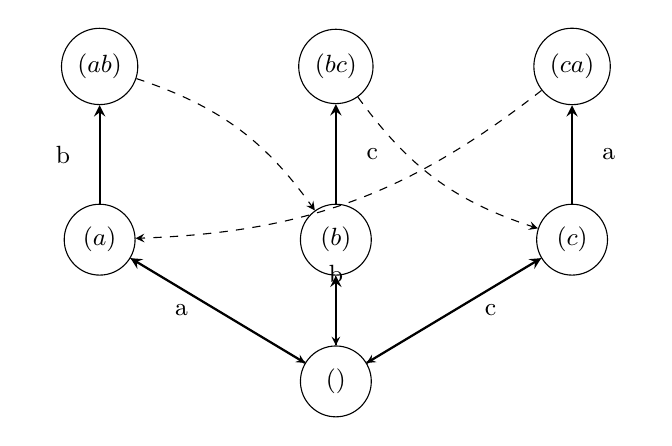
\begin{tikzpicture}[>=stealth, every node/.style={circle, draw, minimum size=9mm, font=\small}]
        \node (root) at (0,0) {$()$};
        \node (a) at (-3,1.8) {$(a)$};
        \node (b) at (0,1.8) {$(b)$};
        \node (c) at (3,1.8) {$(c)$};
        \node (ab) at (-3,4.0) {$(ab)$};
        \node (bc) at (0,4.0) {$(bc)$};
        \node (ca) at (3,4.0) {$(ca)$};

        \draw[->, thick] (root) -- node[left, draw=none] {a} (a);
        \draw[->, thick] (root) -- node[draw=none, above] {b} (b);
        \draw[->, thick] (root) -- node[right, draw=none] {c} (c);
        \draw[->, thick] (a) -- node[left, draw=none] {b} (ab);
        \draw[->, thick] (b) -- node[right, draw=none] {c} (bc);
        \draw[->, thick] (c) -- node[right, draw=none] {a} (ca);

        \draw[->, dashed, bend left=18] (ab) to (b);
        \draw[->, dashed, bend right=18] (bc) to (c);
        \draw[->, dashed, bend left=18] (ca) to (a);
        \draw[->, dashed] (a) -- (root);
        \draw[->, dashed] (b) -- (root);
        \draw[->, dashed] (c) -- (root);
    \end{tikzpicture}
    \caption{Automaton Aho-Corasick dengan failure link yang menghubungkan state ke suffix yang masih valid.}
    \label{fig:aho-automaton}
\end{figure}

Lalu, bagaimana mekanisme pembangunan automatonnya dan bagaimana cara teksnya dipindai? Pada tahap preprocessing, trie akan dibentuk terlebih dahulu, lalu failure link dihitung dengan menelusuri level demi level menggunakan antrian. Setelah automaton siap, teks diproses satu karakter demi satu karakter; jika transisi tidak tersedia, algoritma mengikuti failure link sampai menemukan state yang cocok atau kembali ke akar. Lebih lanjut, algoritma Aho-Corasick dapat dideskripsikan melalui Pseudocode di bawah ini.

\begin{tcolorbox}[breakable,title={Algoritma Aho-Corasick}]
    \begin{algorithmic}[1]
        \Procedure{BuildAutomaton}{$patterns$}
        \State $root \gets$ node baru
        \ForAll{$pattern$ in $patterns$}
        \State sisipkan $pattern$ ke trie dari $root$
        \State tandai node akhir sebagai output pattern
        \EndFor
        \State $queue \gets$ anak-anak langsung dari $root$
        \While{$queue$ tidak kosong}
        \State $v \gets$ pop dari $queue$
        \ForAll{karakter $c$ yang memiliki child dari $v$}
        \State $u \gets child(v, c)$
        \State $f \gets fail(v)$
        \While{$f \neq root$ \textbf{and} child($f$, $c$) tidak ada}
        \State $f \gets fail(f)$
        \EndWhile
        \If{child($f$, $c$) ada}
        \State $fail(u) \gets child(f, c)$
        \Else
        \State $fail(u) \gets root$
        \EndIf
        \State gabungkan output $u$ dengan output $fail(u)$
        \State push $u$ ke $queue$
        \EndFor
        \EndWhile
        \State \Return $root$
        \EndProcedure
        \Statex
        \Procedure{Search}{$text, root$}
        \State $state \gets root$
        \For{$i \gets 0$ to $|text| - 1$}
        \While{$state \neq root$ \textbf{and} child($state$, $text[i]$) tidak ada}
        \State $state \gets fail(state)$
        \EndWhile
        \If{child($state$, $text[i]$) ada}
        \State $state \gets child(state, text[i])$
        \EndIf
        \If{output($state$) tidak kosong}
        \State laporkan seluruh pola pada output($state$) di posisi $i$
        \EndIf
        \EndFor
        \EndProcedure
    \end{algorithmic}
\end{tcolorbox}

Pseudocode di atas menegaskan bahwa kekuatan Aho-Corasick terletak pada pemisahan yang jelas antara pembangunan automaton dan proses pencarian. Setelah trie dan failure link terbentuk, pencarian hanya perlu mengalirkan karakter teks dari kiri ke kanan sambil menjaga state aktif. Karena itu, algoritma ini sangat cocok dibahas setelah komponen trie, failure link, dan output sudah divisualisasikan, sebab pseudocode-nya langsung merefleksikan dua tahap tersebut.

Lebih lanjut, tabel di bawah memperlihatkan bagaimana string \texttt{abccab} dipindai secara bertahap oleh automaton. Pada awalnya automaton bergerak dari akar ke node \texttt{(a)} lalu ke \texttt{(ab)} saat prefiks yang cocok ditemukan. Ketika karakter berikutnya tidak lagi cocok dengan child langsung, algoritma mengikuti failure link ke state yang masih relevan, lalu melanjutkan transisi normal. Di beberapa titik, satu state menghasilkan lebih dari satu output karena node tersebut mewarisi output dari dictionary suffix-nya. Inilah alasan Aho-Corasick mampu menemukan banyak pola sekaligus tanpa memulai pencarian ulang dari akar setiap kali mismatch terjadi.

\begin{table}[H]
    \centering
    \caption{Analysis of input string \texttt{abccab} pada automaton Aho-Corasick.}
    \small
    \setlength{\tabcolsep}{4pt}
    \begin{tabularx}{\textwidth}{>{\raggedright\arraybackslash}p{1.5cm} >{\raggedright\arraybackslash}p{1.8cm} >{\raggedright\arraybackslash}p{2.1cm} >{\raggedright\arraybackslash}X >{\raggedright\arraybackslash}p{3.2cm}}
        \toprule
        Node          & Remaining string & Output:end position & Transition                                                                       & Output                         \\
        \midrule
        \texttt{()}   & \texttt{abccab}  &                     & start at root                                                                    &                                \\
        \texttt{(a)}  & \texttt{bccab}   & \texttt{a:1}        & \texttt{()} to child \texttt{(a)}                                                & Current node                   \\
        \texttt{(ab)} & \texttt{ccab}    & \texttt{ab:2}       & \texttt{(a)} to child \texttt{(ab)}                                              & Current node                   \\
        \texttt{(bc)} & \texttt{cab}     & \texttt{bc:3, c:3}  & \texttt{(ab)} to suffix \texttt{(b)} to child \texttt{(bc)}                      & Current node, Dict suffix node \\
        \texttt{(c)}  & \texttt{ab}      & \texttt{c:4}        & \texttt{(bc)} to suffix \texttt{(c)} to suffix \texttt{()} to child \texttt{(c)} & Current node                   \\
        \texttt{(ca)} & \texttt{b}       & \texttt{a:5}        & \texttt{(c)} to child \texttt{(ca)}                                              & Dict suffix node               \\
        \texttt{(ab)} & \texttt{}        & \texttt{ab:6}       & \texttt{(ca)} to suffix \texttt{(a)} to child \texttt{(ab)}                      & Current node                   \\
        \bottomrule
    \end{tabularx}
\end{table}

Kelebihan utama Aho-Corasick adalah kemampuannya mencari banyak pola sekaligus dengan waktu pencarian linear terhadap panjang teks, sehingga sangat efisien ketika dictionary berisi banyak keyword. Algoritma ini juga deterministik dan stabil karena setiap karakter diproses satu kali dengan bantuan failure link, sehingga cocok untuk pipeline scanning yang butuh hasil konsisten. Di sisi lain, kekurangannya adalah preprocessing yang lebih mahal dibanding pencarian tunggal, memori yang meningkat seiring jumlah state trie, serta kompleksitas implementasi yang lebih tinggi daripada KMP atau Rabin-Karp. Jika jumlah pola sangat kecil, biaya membangun automaton bisa terasa tidak sebanding dengan keuntungan saat pencarian.

Secara kompleksitas, proses pembangunan trie dan failure link memerlukan waktu $O(M)$ dengan $M$ sebagai total panjang semua pola pada implementasi trie yang efisien, sedangkan pencarian teks memerlukan waktu $O(n + z)$ dengan $n$ panjang teks dan $z$ jumlah kemunculan pola yang dilaporkan. Dalam implementasi yang memakai tabel transisi penuh, biaya preprocessing dapat meningkat mengikuti ukuran alfabet dan jumlah state, tetapi pada representasi sparse kompleksitasnya tetap dekat linear terhadap total input pola. Ruang yang dibutuhkan juga bergantung pada jumlah node trie, sehingga secara umum berkisar pada $O(M)$. Karena itu, Aho-Corasick sangat kuat untuk multi-pattern matching dalam skala besar, tetapi trade-off utamanya ada pada kebutuhan memori dan preprocessing yang lebih besar.

\subsection{Algoritma Rabin-Karp}

Rabin-Karp memakai fungsi hash untuk membandingkan pola dengan jendela teks yang bergeser. Selama hash jendela dan hash pola sama, sistem melakukan verifikasi lanjutan terhadap isi string; jika tidak sama, jendela dapat segera dilewati. Pendekatan ini efektif untuk pencarian banyak pola atau ketika hash dapat dihitung ulang secara efisien menggunakan rolling hash \cite{karp1987efficient}.

Secara formal, misalkan teks dinyatakan sebagai $T = t_0 t_1 \dots t_{n-1}$ dan pola sebagai $P = p_0 p_1 \dots p_{m-1}$ dengan $m \leq n$. Rabin-Karp mendefinisikan fungsi hash $h(\cdot)$ atas string sepanjang $m$ dan mencari pergeseran $s$ sehingga $h(P) = h(T[s..s+m-1])$. Agar pencarian efisien, hash jendela berikutnya tidak dihitung dari nol, melainkan diperbarui dengan rolling hash. Secara konseptual, algoritma ini memindahkan beban komparasi dari perbandingan karakter penuh ke perbandingan nilai hash yang jauh lebih murah, lalu hanya melakukan verifikasi karakter ketika hash memang cocok.

Komponen utama Rabin-Karp terdiri dari tiga bagian yang saling bergantung. Pertama, ada hash pola yang dihitung sekali pada awal preprocessing. Kedua, ada hash jendela teks yang selalu mewakili substring sepanjang $m$ dari teks utama. Ketiga, ada mekanisme rolling hash yang memperbarui nilai hash ketika jendela bergeser satu posisi ke kanan. Jika hash cocok, algoritma melakukan pemeriksaan ulang karakter demi karakter untuk memastikan bahwa kecocokan tersebut bukan collision. Karena itu, visualisasi Rabin-Karp paling mudah dipahami sebagai kombinasi antara pola, jendela teks, dan pembaruan hash yang terus bergerak.

\begin{figure}[H]
    \centering
    \begin{tikzpicture}[>=stealth, node distance=2.2cm and 2.8cm, every node/.style={draw, rounded corners, align=center, font=\small, minimum width=2.8cm, minimum height=1cm}]
        \node (pattern) {Pola $P$\\\texttt{aba}};
        \node (phash) [right=of pattern] {Hash pola\\$h(P)$};
        \node (window) [below=of pattern] {Jendela teks\\$T[s..s+m-1]$};
        \node (whash) [right=of window] {Hash jendela\\$h(T[s..s+m-1])$};
        \node (check) [below=of whash] {Verifikasi karakter\\jika hash cocok};

        \draw[->, thick] (pattern) -- (phash);
        \draw[->, thick] (window) -- (whash);
        \draw[->, thick] (phash) -- node[right, draw=none] {bandingkan} (whash);
        \draw[->, thick] (whash) -- (check);
        \draw[->, thick] (check.west) .. controls +(-2,0) and +(0,-1) .. node[below left=2mm and 2mm, draw=none] {rolling hash\\jendela berikutnya} (window.south);
    \end{tikzpicture}
    \caption{Komponen utama Rabin-Karp: hash pola, hash jendela teks, rolling hash, dan verifikasi karakter ketika hash cocok.}
    \label{fig:rk-components}
\end{figure}

Setelah hash pola dihitung, setiap jendela teks dibandingkan melalui hash terlebih dahulu; bila hash tidak sama, jendela langsung digeser tanpa komparasi karakter tambahan. Jika hash sama, barulah algoritma memeriksa isi substring untuk memastikan bahwa kecocokan tersebut benar-benar valid. Alur inilah yang membuat pseudocode Rabin-Karp menjadi ringkas namun sangat representatif terhadap proses pencarian berbasis hash.

\begin{tcolorbox}[breakable,title={Algoritma Rabin-Karp}]
    \begin{algorithmic}[1]
        \Procedure{RabinKarpSearch}{$text, pattern$}
        \State $n \gets \text{length}(text)$
        \State $m \gets \text{length}(pattern)$
        \State $q \gets$ bilangan prima untuk modulus
        \State $d \gets$ ukuran alfabet / basis hash
        \State $hP \gets$ \Call{Hash}{$pattern, d, q$}
        \State $hW \gets$ \Call{Hash}{$text[0..m-1], d, q$}
        \State $power \gets d^{m-1} \bmod q$
        \For{$s \gets 0$ to $n - m$}
        \If{$hP = hW$}
        \If{$text[s..s+m-1] = pattern$}
        \State \textbf{report match} at shift $s$
        \EndIf
        \EndIf
        \If{$s < n - m$}
        \State $hW \gets$ rolling hash untuk jendela berikutnya
        \EndIf
        \EndFor
        \EndProcedure
    \end{algorithmic}
\end{tcolorbox}

Pseudocode di atas menekankan bahwa Rabin-Karp tidak langsung membandingkan seluruh karakter pada setiap pergeseran. Sebaliknya, algoritma ini terlebih dahulu memeriksa kesetaraan hash, lalu hanya melakukan pemeriksaan string penuh ketika hash tersebut cocok. Karena itu, pseudocode menjadi masuk akal setelah pembahasan komponen hash pola, hash jendela, dan rolling hash selesai dijelaskan.

Sebagai ilustrasi, algoritma Rabin-Karp dapat digunakan untuk mencari pola \texttt{aba} di dalam teks \texttt{abacaba}. Pada contoh ini, jendela teks bergeser satu karakter demi satu karakter dengan panjang yang sama seperti pola. Hash jendela pertama dan hash pola dibandingkan terlebih dahulu; jika hash tidak sama, jendela langsung dilewati, sedangkan jika hash sama maka substring diverifikasi secara karakter demi karakter. Ilustrasi berikut menunjukkan proses tersebut secara bertahap.

\begin{table}[H]
    \centering
    \caption{Contoh langkah pencocokan Rabin-Karp pada teks \texttt{abacaba} dengan pola \texttt{aba}.}
    \small
    \setlength{\tabcolsep}{4pt}
    \begin{tabularx}{\textwidth}{c c c c >{\raggedright\arraybackslash}X}
        \toprule
        Langkah & Shift $s$ & Window teks  & Hash dibandingkan           & Keputusan                         \\
        \midrule
        1       & 0         & \texttt{aba} & $h(\texttt{aba}) = h(P)$    & Verifikasi cocok, match ditemukan \\
        2       & 1         & \texttt{bac} & $h(\texttt{bac}) \neq h(P)$ & Langsung geser, tanpa verifikasi  \\
        3       & 2         & \texttt{aca} & $h(\texttt{aca}) \neq h(P)$ & Langsung geser, tanpa verifikasi  \\
        4       & 3         & \texttt{cab} & $h(\texttt{cab}) \neq h(P)$ & Langsung geser, tanpa verifikasi  \\
        5       & 4         & \texttt{aba} & $h(\texttt{aba}) = h(P)$    & Verifikasi cocok, match ditemukan \\
        \bottomrule
    \end{tabularx}
\end{table}

Contoh di atas memperlihatkan bahwa Rabin-Karp bekerja dengan memindahkan fokus dari komparasi karakter penuh ke komparasi hash jendela. Ketika hash cocok, barulah substring diperiksa ulang untuk memastikan tidak terjadi collision. Pada teks yang panjang dengan banyak jendela yang tidak cocok, pendekatan ini bisa sangat efisien karena sebagian besar pergeseran hanya membutuhkan pembaruan hash, bukan komparasi ulang seluruh karakter.

Kelebihan utama Rabin-Karp adalah kemampuannya menangani pencarian banyak pola atau pencarian berbasis rolling hash dengan biaya rata-rata yang efisien. Algoritma ini juga mudah diperluas karena inti logikanya sederhana: hitung hash, bandingkan, lalu verifikasi jika perlu. Di sisi lain, kekurangannya adalah adanya collision; dua string berbeda dapat saja memiliki hash yang sama sehingga verifikasi tetap diperlukan. Selain itu, jika rolling hash atau modulus yang dipilih kurang baik, performa praktisnya dapat menurun karena terlalu banyak collision atau distribusi hash yang tidak merata. Dengan demikian, Rabin-Karp kuat untuk implementasi yang mengandalkan hashing, tetapi kualitas hash menjadi faktor yang sangat menentukan.

Secara kompleksitas, preprocessing hash pola memerlukan waktu $O(m)$ dan pembaruan rolling hash untuk setiap pergeseran juga dapat dilakukan dalam $O(1)$, sehingga pencarian rata-rata biasanya berada di sekitar $O(n + m)$. Namun, pada kasus terburuk ketika collision sering terjadi, Rabin-Karp dapat turun menjadi $O(nm)$ karena verifikasi karakter penuh dilakukan pada banyak jendela. Ruang tambahannya sendiri kecil, umumnya $O(1)$ selain penyimpanan input. Kompleksitas ini menjadikan Rabin-Karp menarik karena sangat sederhana secara konsep, tetapi tetap bergantung pada kualitas fungsi hash dan probabilitas collision yang muncul pada data.

\section{Regular Expression (\texttt{RegEx}) Matching}

Regular expression adalah notasi formal untuk mendeskripsikan bahasa reguler, yaitu himpunan string yang dapat dibangun dari alfabet tertentu melalui operasi bahasa formal. Dalam teori automata, sebuah regex tidak hanya dianggap sebagai sintaks pencarian string, tetapi juga sebagai representasi aljabar dari language yang dibentuk oleh simbol dasar, operasi union, concatenation, dan Kleene star \cite{hopcroft2006automata}.

Secara formal, misalkan $\Sigma$ adalah alfabet. Definisi regex dapat dibangun secara rekursif sebagai berikut. $\emptyset$, $\varepsilon$, dan setiap simbol $a \in \Sigma$ adalah regular expression. Jika $r$ dan $s$ adalah regular expression, maka operasi formal utamanya adalah

\begin{enumerate}
    \item $r + s$ atau $r \mid s$, yaitu \textit{union}, yang membentuk language berisi string dari salah satu komponen.
    \item $rs$, yaitu \textit{concatenation}, yang membentuk string dengan bahasa pertama diikuti bahasa kedua.
    \item $r^*$, yaitu \textit{Kleene star}, yang membentuk semua pengulangan nol kali atau lebih dari bahasa dasar.
    \item $r^+$, yaitu satu atau lebih pengulangan dari bahasa dasar.
    \item $r?$ , yaitu bentuk opsional yang menerima nol atau satu kemunculan.
\end{enumerate}

Setiap regex $r$ merepresentasikan language $L(r)$, yaitu himpunan semua string yang diterima oleh ekspresi tersebut. Hubungan ini menjadikan RegEx sebagai bentuk ringkas untuk mendeskripsikan pola string tanpa menuliskan seluruh kemungkinan string secara eksplisit \cite{hopcroft2006automata,mdnregexp}. Pada implementasi praktis, operasi seperti grouping dengan kurung, character class, anchor, dan quantifier memperluas ekspresi formal ini ke notasi yang lebih ergonomis untuk pencocokan teks. Karena itu, aturan sintaks RegEx modern sebenarnya tetap berakar pada operasi formal bahasa reguler.


Pada aplikasi ini, RegEx relevan untuk menangkap pola seperti kata yang diikuti angka, misalnya bentuk yang sengaja dimodifikasi agar tidak sama persis dengan keyword di daftar utama. Dibandingkan exact matching, pendekatan ini lebih fleksibel, tetapi perlu dibatasi dengan hati-hati agar tidak menghasilkan terlalu banyak false positive. Dengan kata lain, RegEx dipakai ketika sistem ingin mengekspresikan pola secara lebih umum daripada daftar kata kunci statis.

Contoh regex sederhana adalah \texttt{a\*b}, yang menerima string \texttt{b}, \texttt{ab}, \texttt{aab}, dan \texttt{aaab}, karena simbol \texttt{a} boleh muncul nol kali atau lebih sebelum \texttt{b}. Contoh lainnya adalah \texttt{(ab)+}, yang menerima \texttt{ab}, \texttt{abab}, dan \texttt{ababab}. Contoh yang lebih kompleks adalah \texttt{[A-Za-z]+\textbackslash d{2,3}}, yang dapat mencocokkan string seperti \texttt{MAXWIN99}, \texttt{slot123}, atau \texttt{Bonus202}, karena pola tersebut meminta satu atau lebih huruf yang diikuti dua sampai tiga digit. Untuk contoh berbasis anchor, regex \texttt{\^gacor\$} hanya menerima string \texttt{gacor} tanpa karakter tambahan di depan atau belakang.


\section{Fuzzy Matching}

Fuzzy matching adalah pendekatan pencocokan yang tidak menuntut identitas string secara penuh, melainkan menerima derajat kemiripan tertentu. Teknik ini cocok digunakan ketika data mengandung noise, variasi ejaan, atau manipulasi karakter visual-similar. Dalam literatur pencocokan string, ide ini sangat erat dengan pengukuran jarak edit, terutama Levenshtein distance \cite{levenshtein1966binary}.

Untuk memperjelas konsep ini, pada Gambar~\ref{fig:fuzzy-matching-example} ditunjukkan contoh visualisasi proses fuzzy matching. Gambar memperlihatkan dua string yang dibandingkan beserta operasi edit (insertion, deletion, substitution) yang diperlukan untuk mengubah satu string menjadi lainnya. Pada implementasi praktis, tiap operasi dapat diberi bobot berbeda (mis. substitution visual-similar diberi penalti lebih kecil), lalu jarak edit total dibandingkan dengan ambang (threshold) untuk menentukan apakah dua string dianggap "cocok".

\begin{figure}[H]
    \centering
    
\includegraphics[width=0.75\linewidth]{fuzzy-matching.png}
    \caption{Contoh visualisasi fuzzy matching: operasi insertion, deletion, dan substitution serta penentuan jarak edit.}
    \label{fig:fuzzy-matching-example}
\end{figure}

\subsection{Weighted Levenshtein Distance}
Weighted Levenshtein distance memperluas jarak edit standar dengan memberikan bobot berbeda pada operasi insertion, deletion, dan substitution. Pendekatan ini memungkinkan penalti substitution yang lebih kecil untuk pasangan karakter yang mirip secara visual (Contohnya, \texttt{o} vs  \texttt{0} dan \texttt{l} vs \texttt{1}), sehingga sistem menjadi lebih toleran terhadap variasi yang sering muncul pada data nyata \cite{levenshtein1966binary}.

Lebih formal, misalkan $s = s_1 s_2 \dots s_m$ dan $t = t_1 t_2 \dots t_n$ adalah dua string. Definisikan fungsi biaya
\(w_{ins}(c)\) untuk menyisipkan karakter $c$, \(w_{del}(c)\) untuk menghapus karakter $c$, dan \(w_{sub}(a,b)\) untuk mengganti karakter $a$ menjadi $b$. Selain itu, definisikan pula matriks biaya $D(i,j)$ sebagai biaya minimum untuk mengubah prefix $s_{1..i}$ menjadi $t_{1..j}$. Inisialisasi dan rekurensi dasar adalah
$$
    D(0,0)=0,\qquad D(i,0)=D(i-1,0)+w_{del}(s_i),\qquad D(0,j)=D(0,j-1)+w_{ins}(t_j).
$$
Untuk $i\ge1, j\ge1$ akan berlaku
$$
    D(i,j)=\min\begin{cases}
        D(i-1,j)+w_{del}(s_i), \\
        D(i,j-1)+w_{ins}(t_j), \\
        D(i-1,j-1)+\begin{cases}0 &\text{jika } s_i=t_j,\\ w_{sub}(s_i,t_j) &\text{lainnya.}\end{cases}
    \end{cases}
$$

Secara intuitif, rumus tersebut sedang memilih operasi edit termurah pada setiap pasangan prefix. Cabang pertama berarti karakter terakhir dari string sumber dihapus, cabang kedua berarti karakter terakhir dari string target disisipkan, dan cabang ketiga berarti kedua karakter terakhir dibandingkan langsung, lalu diberi biaya nol jika sama atau biaya substitution jika berbeda. Dengan kata lain, algoritma ini membangun solusi dari potongan kecil ke potongan yang lebih besar sambil selalu menyimpan pilihan termurah yang pernah ditemukan.

Secara alternatif, dengan notasi \(\mathrm{head}(x)\) dan \(\mathrm{tail}(x)\), untuk string non-kosong, definisi dapat ditulis sebagai
$$
    \mathrm{lev}(a,b)=\begin{cases}
        \sum_{c\in a} w_{del}(c)                                                                                 & \text{jika } |b|=0,                             \\
        \sum_{c\in b} w_{ins}(c)                                                                                 & \text{jika } |a|=0,                             \\
        \mathrm{lev}(\mathrm{tail}(a),\mathrm{tail}(b))                                                          & \text{jika } \mathrm{head}(a)=\mathrm{head}(b), \\
        \min\left\{\begin{array}{l}
                       w_{ins}(\mathrm{head}(b))+\mathrm{lev}(a,\mathrm{tail}(b)), \\
                       w_{del}(\mathrm{head}(a))+\mathrm{lev}(\mathrm{tail}(a),b), \\
                       w_{sub}(\mathrm{head}(a),\mathrm{head}(b))+\mathrm{lev}(\mathrm{tail}(a),\mathrm{tail}(b))
                   \end{array}\right. & \text{lainnya.}
    \end{cases}
$$

Contoh, ambil $a=\texttt{o}$ dan $b=\texttt{0}$ serta biaya $w_{ins}=1$, $w_{del}=1$, $w_{sub}('o','0')=0.3$. Pada kasus ini, intuitifnya kita hanya perlu satu langkah substitusi kecil karena kedua karakter hampir sama secara visual, sehingga sistem lebih memilih jalur diagonal daripada menghapus lalu menyisipkan ulang karakter. Maka,
\begin{align*}
    \mathrm{lev}('', '')  & = 0,                               \\
    \mathrm{lev}('', '0') & = 1,                               \\
    \mathrm{lev}('o', '') & = 1,                               \\
    \mathrm{lev}('o','0') & = \min\{1+1,\;1+1,\;0+0.3\} = 0.3.
\end{align*}

Hasil tersebut menunjukkan bahwa substitusi antara karakter visual-similar mendapat penalti lebih kecil sehingga jarak akhir turun, yang berguna untuk mendeteksi manipulasi karakter ringan tanpa menaikkan false positive secara signifikan.

\section{Optical Character Recognition (OCR)}

Optical Character Recognition adalah proses mengekstrak teks dari citra atau gambar sehingga isi visual dapat diperlakukan sebagai teks yang dapat dicari. OCR penting ketika konten yang ingin diperiksa tidak muncul langsung sebagai DOM text, melainkan tertanam di dalam gambar. Ray Smith menjelaskan bahwa Tesseract dibangun sebagai mesin OCR yang mampu melakukan pengenalan karakter melalui pipeline analisis citra dan interpretasi teks \cite{smith2007tesseract}.

Dalam konteks program, OCR berfungsi sebagai lapisan tambahan setelah pemindaian teks biasa. Setelah teks diekstrak dari gambar, hasilnya masih perlu diproses dengan mekanisme pencocokan yang sama agar deteksi tetap konsisten dengan keyword yang digunakan pada halaman.

\section{Chromium Browser Extension}

Chromium browser extension adalah perangkat lunak tambahan yang berjalan di atas browser Chromium untuk memperluas perilaku halaman web tanpa memodifikasi browser itu sendiri. Dokumentasi resmi Chrome Extensions menjelaskan bahwa extension umumnya tersusun dari komponen seperti background script, content script, dan UI permukaan seperti popup atau side panel, masing-masing dengan tanggung jawab yang berbeda \cite{chromeextdocs}.

Pada arsitektur semacam ini, content script biasanya bertugas membaca dan memanipulasi halaman aktif, background script mengelola pesan dan state yang lebih global, sedangkan popup memberi antarmuka interaksi kepada pengguna. Pemisahan tanggung jawab tersebut membuat extension lebih mudah diatur ketika harus melakukan scan, menyimpan statistik, dan memberi umpan balik visual di halaman.

\subsection{Arsitektur Singkat}

Arsitektur singkat extension ini terdiri dari tiga lapisan utama. Pertama, 	extit{content script} berjalan pada setiap halaman aktif dan menjadi mesin utama deteksi: ia membaca teks DOM, mengumpulkan target pencarian, menjalankan rangkaian algoritma pattern matching, memberi highlight/blur pada elemen yang cocok, serta menjalankan OCR untuk elemen gambar bila opsi OCR diaktifkan. Kedua, 	extit{popup} berperan sebagai panel kendali yang menampilkan statistik hasil scan, tombol pemindaian manual, dan toggle fitur seperti blur serta OCR. Ketiga, 	extit{background service worker} menangani state yang bersifat global, terutama badge pada ikon extension dan sinkronisasi nilai di 	exttt{chrome.storage}. Dengan pembagian ini, proses deteksi tetap dapat berjalan di halaman aktif, sementara antarmuka pengguna tetap ringan dan status hasil tetap konsisten lintas tab serta sesi.

Secara alur, popup mengirimkan permintaan scan ke content script melalui 	exttt{chrome.tabs.sendMessage}. Content script kemudian membentuk konteks scan dari URL dan teks halaman, menjalankan mesin deteksi, menyimpan ringkasan statistik ke storage lokal, lalu mengirimkan hasil visual kembali ke halaman melalui highlight dan blur. Background mendengarkan perubahan pada 	exttt{chrome.storage.local} untuk memperbarui badge angka pada ikon extension, sehingga pengguna dapat melihat adanya temuan bahkan sebelum membuka popup.

\begin{figure}[H]
    \centering
    \begin{tikzpicture}[
            >=stealth,
            node distance=2.2cm and 2.8cm,
            box/.style={draw, rounded corners, align=center, font=\small, minimum width=3.2cm, minimum height=1.05cm},
            arrow/.style={->, thick}
        ]
        \node[box] (popup) {Popup UI\\\textit{Scan now}, toggle blur, toggle OCR\\render statistik};
        \node[box, right=of popup] (content) {Content Script\\scan DOM, pattern matching, OCR\\highlight / blur elemen};
        \node[box, below=of content] (storage) {\texttt{chrome.storage.local}\\statistik, status fitur};
        \node[box, left=of storage] (background) {Background Service Worker\\badge ikon, sync state};
        \node[box, above=of content] (page) {Halaman Aktif\\teks DOM, gambar, elemen target};

        \draw[arrow] (popup) -- node[above, draw=none] {\texttt{scan-now}} (content);
        \draw[arrow] (content) -- node[right, draw=none] {baca} (page);
        \draw[arrow] (content) -- node[right, draw=none] {simpan hasil} (storage);
        \draw[arrow] (storage) -- node[below, draw=none] {\texttt{onChanged}} (background);
        \draw[arrow] (background) -- node[left, draw=none] {badge} (popup);
        \draw[arrow] (popup) -- node[left, draw=none] {toggle fitur} (storage);
    \end{tikzpicture}
    \caption{Arsitektur singkat \texttt{Judol Detector}: popup menjadi pusat kontrol, content script menjalankan deteksi pada halaman aktif, dan background menjaga badge serta sinkronisasi state.}
    \label{fig:judol-extension-architecture}
\end{figure}

\subsection{Akuisisi dan Pemindaian DOM}

Akuisisi DOM pada program ini memakai pendekatan \textit{hybrid scan}. Bagian teks dikumpulkan dengan menelusuri \texttt{Text node} melalui \texttt{TreeWalker}, lalu setiap node dipetakan ke elemen kontainer yang paling representatif. Selama proses ini, elemen skrip dan gaya seperti \texttt{script}, \texttt{style}, \texttt{noscript}, \texttt{meta}, dan \texttt{link} diabaikan, begitu pula elemen yang tidak terlihat atau yang berada di dalam UI internal extension. Bagian gambar dipindai terpisah dengan menelusuri semua elemen \texttt{img}, memeriksa apakah elemen tersebut terlihat, menghindari sumber gambar yang tidak relevan, lalu memakai \texttt{alt} atau \texttt{title} sebagai konteks teks tambahan. Pendekatan dua jalur ini membuat sistem dapat menangani teks biasa dan konten visual secara lebih stabil tanpa mencampur keduanya.

Setelah target teks dan gambar terkumpul, sistem membangun konteks scan yang berisi URL halaman, teks normalisasi, dan daftar target yang sudah difilter. Konteks ini kemudian dikirim ke mesin deteksi pattern matching. Jika sebuah elemen cocok, sistem tidak hanya menandai elemen tersebut, tetapi juga menyimpan indeks target agar hasil highlight, tooltip, dan perhitungan statistik dapat dilacak kembali secara konsisten.

Secara ringkas, alur pemindaian DOM pada program ini dapat dituliskan sebagai berikut.

\begin{enumerate}
    \item Telusuri seluruh node teks pada halaman yang terlihat dan bukan bagian dari UI internal extension.
    \item Peta setiap node teks ke kontainer yang paling representatif, lalu simpan hanya kontainer yang belum pernah diproses.
    \item Telusuri seluruh elemen gambar yang terlihat dan memiliki sumber valid.
    \item Abaikan elemen duplikat serta sumber gambar yang sudah pernah diproses.
    \item Bentuk konteks scan dari URL halaman, teks hasil normalisasi, dan daftar target teks serta gambar.
    \item Kirim konteks tersebut ke modul deteksi untuk menghasilkan highlight, tooltip, dan statistik.
\end{enumerate}